%!TeX root=../Monografia - Mikhael Pinto.tex
%("dica" para o editor de texto: este arquivo é parte de um documento maior)

% Conteúdo da subseção sobre Notificações
% Este arquivo é importado em 02-implementacao.tex

%acho que teve comunicação nas coortes%
Com 1.217 participantes distribuídos geograficamente por São Paulo e engajados em experimento com rotação semanal de coortes, estabelecer canal eficaz de comunicação mostrou-se crítico. Eventos requerendo notificação incluíam: início de nova coorte (informar mudança de remuneração), disponibilidade de pagamento (créditos depositados no Bilhete Único), manutenções programadas no sistema, lembretes de preenchimento de questionários qualitativos, e esclarecimentos sobre regras do experimento após dúvidas recorrentes. Sistema de notificações implementado no painel oferece dois canais simultâneos: push notifications via Firebase Cloud Messaging (FCM) para aplicativo Android, e email via SMTP (Gmail) para endereços cadastrados.

A interface oferece três estratégias de direcionamento: (i) envio individual para IDs específicos separados por vírgula (ex: comunicação de suporte técnico, ``participantes 123, 456 e 789: problema reportado foi corrigido''); (ii) envio por coorte via IDs de grupos experimentais (ex: ``participantes da coorte 2: esta semana sua remuneração é R\$~0,60/km''); e (iii) broadcast para todos participantes cadastrados (ex: ``sistema em manutenção dia 15 das 02h-04h''). Esta granularidade atende necessidades distintas: comunicação individualizada reduz ruído para participantes não afetados; segmentação por coorte mantém integridade do desenho experimental (evitando confusão sobre qual valor de remuneração aplica-se a cada grupo); broadcast garante que informações críticas alcancem todos.

O formulário de criação requer título (usado como assunto de email e cabeçalho de push notification) e corpo da mensagem. Campo de corpo aceita HTML completo, permitindo formatação rica em emails: parágrafos (\texttt{<p>}), quebras de linha (\texttt{<br>}), negrito (\texttt{<strong>}), listas, e links. Suporte a HTML mostrou-se valioso para comunicações longas ou complexas, como FAQ respondendo dúvidas recorrentes ou instruções passo-a-passo para resolver problemas comuns. Push notifications, devido a limitações de espaço em dispositivos móveis, exibem apenas texto plano, adequado para mensagens concisas. Checkbox independentes para cada canal (push e/ou email) permitem escolher meio mais apropriado: push para alertas urgentes que requerem atenção imediata; email para informações detalhadas que usuário pode consultar posteriormente. A Figura~\ref{fig:notificacao_criar} mostra a interface de criação.

 \begin{figure}[htb]
   \centering
   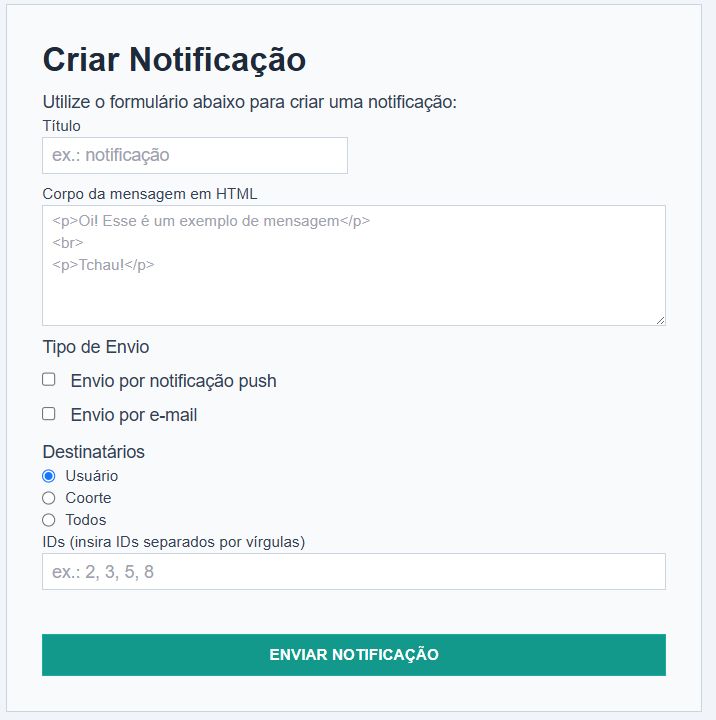
\includegraphics[width=0.95\textwidth]{figuras/notificacao_criar.PNG}
   \caption{Formulário de criação e envio de notificações para participantes.}
   \label{fig:notificacao_criar}
 \end{figure}

Para push notifications, o sistema consulta tabela de tokens FCM associados a cada participante (registrados durante primeira abertura do aplicativo), envia payload via API do Firebase, e notificação aparece na bandeja de notificações Android do participante. Falhas ocasionais ocorrem quando aplicativo é desinstalado ou token expira. Para emails, sistema busca endereços cadastrados, envia via protocolo SMTP autenticado em conta Gmail institucional, posicionando destinatários em BCC (cópia oculta para privacidade) e destinatário padrão configurável (tipicamente \texttt{bikesp-app@ime.usp.br}) no campo ``Para''. Esta arquitetura preserva privacidade (nenhum participante vê emails de outros) e profissionalismo (remetente institucional aumenta confiabilidade, reduzindo classificação como spam).

A funcionalidade de cópia oculta para email do administrador que enviou a notificação (mencionada em documentação como ``enviadas em cópia oculta para o email do administrador'') cria trilha de auditoria e permite verificação imediata de conteúdo e destinatários. Este registro mostrou-se útil para resolver disputas e manter histórico de comunicações para análise de engajamento.

O sistema valida que ao menos um canal (push ou email) está selecionado; que IDs de usuários/coortes são numéricos; e que campo de IDs é obrigatório apenas quando estratégia ``Usuário'' ou ``Coorte'' está selecionada (e escondida quando ``Todos'' marcado). Log de todas operações registra quem enviou, para quem, quando, e conteúdo da mensagem.

O sistema de notificações foi utilizado para diversos fins: broadcasts (anúncios gerais, disponibilidade de pagamentos), notificações por coorte (lembretes de remuneração ativa, instruções específicas), e mensagens individuais (suporte técnico, correções de problemas).


